%!TEX root = ../../main.tex

\section{Reactive Synthesis from Extended Bounded Response LTL}
\label{sec:ebr-ltl-synthesis}

At this point we have reached the end of our journey. To sum up what we have explained so far, but also to see a practical use of them, let us have a look at the approach presented in \cite{geatti-2020-08} to reactive synthesis from $\ebrltl$ formulas. Note that we will give a brief indication of the whole procedure just to introduce the most important concepts. If you are interested in learning more about that, read the paper.

In \cite{geatti-2020-08} has been investigated a procedure to build the respective safety arena from any $\ebrltl$ formula.
In particular, the input of the procedure is a $\ebrltl$ formula, while the output is the Deterministic Symbolic Safety Automaton in extended AIGER format for reactive synthesis. In order to understand the whole procedure, we need to introduce some concepts: Safety Symbolic Automata, $Past\ebrltl$ and canonical $Past\ebrltl$.

In symbolic automata, states are identified by the value of state variables, and both initial and accepting states and the transition relation are represented as Boolean formulas. This allows them to be exponentially more succinct than equivalent explicitly represented automata. The transition relation $T(X,\Sigma,X')$ is built over states variables, input variables and a primed version of state variables representing the values of state variables st the next state.
A Symbolic Safety Automaton is a Safety Automaton where the states are represented symbolically.
For reactive synthesis, a crucial property of an automaton $\automaton$ is determinism, since in order to check if $\sigma \in \omegalang{(\automaton)}$ it suffices to check if the trace induced by $\sigma$ in $\automaton$ is accepting. For this reason we require that each SSA is deterministic.
Notice, this implies that for each $\sigma \in (2^\Sigma)^\omega$, there exists exactly one trace induced by $\sigma$ for any given Deterministic SSA. 

$Past\ebrltl$ is a logic equivalent to $\ebrltl$ which is easier to be converted in a corresponding canonical form (canonical $Past\ebrltl$) not containing nested occurrences of unbounded temporal operators, whose operands can be only full-past formulas and each of these is prefixed by an arbitrary number of next operators.

\begin{definition}[\cite{geatti-2020-08} Symbolic Safety Automata (SSA)]
A SSA is a tuple $\automaton = \tuple{V,I,T,S}$, where: (i) $V = X \cup \Sigma$ is a set of state variables and $\Sigma$ is a set of input variables; (ii) $I(X)$ is the set of initial states; (iii) $T(X,\Sigma,X')$ the transition relation; (iv) $S(X)$ the set of safe states.
\end{definition}

\begin{definition}[\cite{geatti-2020-08} Acceptance of SSA]
Let $\automaton$ be a SSA. 
A trace is a sequence $\tau  = \sequence{\tau_0,\tau_1,\dots} \in (2^V)^\omega$ of subsets $\tau_i$ of $V$ that satisfies the transition relation of $\automaton$, that is, such that for all $i \geq 0$, $T(X,\Sigma,X')$ is satisfied when $\tau_i$ is used to interpret variables from $X$ and $\Sigma$, and $\tau_{i+1}$ is used to interpret variables from $X'$. 
We say that a trace $\tau$ is induced by a word $\sigma = \sequence{\sigma_0,\sigma_1,\dots} \in (2^\Sigma)^\omega$ if and only if $\sigma_i = \tau_i \cap \Sigma$ for all $i \geq 0$.
A trace $\tau$ is accepting (or safe) if and only if $\tau_i$ satisfies $S(X)$ for all $i \geq 0$. 
The language of $\automaton$, denoted as $\lang{\automaton}$, is the set of all $\sigma \in (2^\Sigma)^\omega$ such that there exists an accepting trace induced by $\sigma$ in $\automaton$. 
\end{definition}

\begin{definition}[\cite{geatti-2020-08} Deterministic SSA]
A SSA $\automaton = \tuple{V,I,T,S}$ is deterministic if: (i) the formula $I$ has exactly one satisfying assignment; (ii) the transition relation is of the form $T(X,\Sigma,X') := \bigwedge_{x \in X} (x' \iff \beta_x(X \cup \Sigma))$, where each $\beta_x(X \cup \Sigma)$ is a Boolean formula over $X$ and $\Sigma$.
\end{definition}

\begin{definition}[\cite{geatti-2020-08} The logic $Past\ebrltl$] \label{def:past-ebrltl}
A $Past\ebrltl$ formula $\chi$ is inductively defined as follows:
\begin{flalign*}
&\psi    := p \; | \; \ltlNeg{\psi} \; | \; \ltlOr{\psi_1}{\psi_2} \; | \; \ltlY{\psi} \; | \; \ltlS{\psi_1}{\psi_2} \\
&\phi    := \psi \; | \; \ltlAnd{\phi_1}{\phi_2} \; | \; \ltlX{\phi} \; | \; \ltlG{\phi} \; | \; \ltlR{\ltlXexp{\psi}{i}}{\phi} \\
&\chi    := \lambda \; | \; \ltlOr{\chi_1}{\chi_2} \; | \; \ltlAnd{\chi_1}{\chi_2}
\end{flalign*}
\end{definition}

\begin{definition}[\cite{geatti-2020-08} Canonical $Past\ebrltl$] \label{def:canonical-past-ebrltl}
The \textit{canonical form} of $Past\ebrltl$ formulas is inductively defined as follows:
\begin{flalign*}
&\psi    := p \; | \; \ltlNeg{\psi} \; | \; \ltlOr{\psi_1}{\psi_2} \; | \; \ltlY{\psi} \; | \; \ltlS{\psi_1}{\psi_2} \\
&\phi    := \psi \; | \; \ltlG{\psi} \; | \; \ltlR{\psi_1}{\psi_2} \\
&\lambda := \phi \; | \; \ltlX{\lambda} \\
&\chi    := \lambda \; | \; \ltlOr{\chi_1}{\chi_2} \; | \; \ltlAnd{\chi_1}{\chi_2}
\end{flalign*}
\end{definition}

The transformation of $\ebrltl$ formulas into deterministic SSAs consists of three steps and the whole procedure is depicted in \autoref{fig:ebr-ltl-synthesis-procedure}:
\begin{itemize}
    \item a translation from $\ebrltl$ to $\pastebrltl$;
    \item a translation from $\pastebrltl$ to its canonical form;
    \item a transformation of canonical $\pastebrltl$ formulas into deterministic SSAs. 
\end{itemize}

\begin{figure}[!htp]
    \centering
    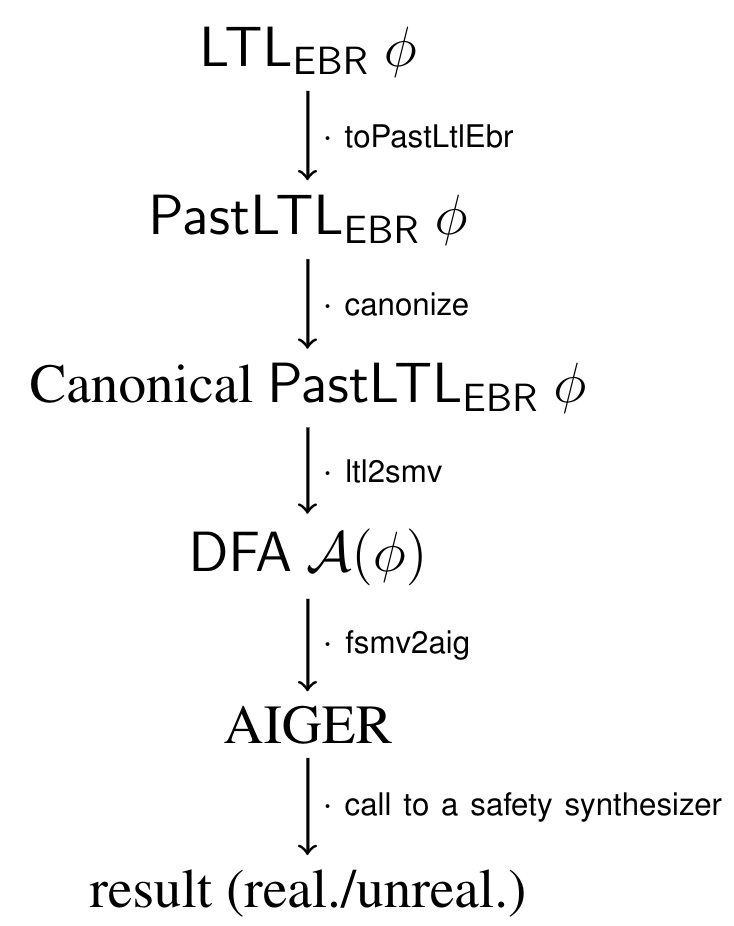
\includegraphics[width=0.4\linewidth]{figures/ebr-ltl-synthesis.png}
    \caption{\cite{geatti-2020-08} The overall procedure to synthesize a $\ebrltl$ formula}
    \label{fig:ebr-ltl-synthesis-procedure}
\end{figure}

The first step consists in translating each $\fpltl$ sub-formula in $\phi$ formula $\ebrltl$ into an equivalent one, which is of the form $\ltlXexp{\psi}{d}$, with $\psi \in \fpltl$ and $d \in \Nat$. This process is called pastification and is useful because full-past formulas can be represented by deterministic monitors, since "the past has already happened".

\begin{proposition}[\cite{geatti-2020-08} Soundness of pastification]
Let $\phi$ be a $\fbltl$ formula. For all state sequences $\sigma \in (2^\Sigma)^\omega$, all $i \in \Nat$ and all $d \geq D(\phi)$, it holds that
\begin{flalign*}
\sigma,i \models \phi \iff \sigma,i \models \ltlXexp{\Pi(\phi,d)}{d}
\end{flalign*}
\end{proposition}

The second step is the canonization of the $Past\ebrltl$ formula obtained from the previous step, in order to obtain an equivalent formula in canonical form. 
Canonical $Past\ebrltl$ formulas are Boolean combinations of formulas of the form $\ltlXexp{\psi_1}{i}$, $\ltlXexp{\ltlG{\psi_1}}{i}$, $\ltlXexp{\ltlR{\psi_1}{\psi_2}}{i}$, where $\psi_1$ and $\psi_2$ are full past formulas. 
Compared to general $Past\ebrltl$ formulas, formulas in canonical form do not admit neither nested unbounded operators nor next operators in front of the left-hand argument of a \textit{release}. The canonization of a $Past\ebrltl$ formula is obtained by applying a set of rewriting rules.
The particular shape of canonical $Past\ebrltl$ formulas makes it possible to encode the specifications into deterministic SSAs. The key observation is that $\fpltl$ formulas can be encoded into deterministic automata since these formulas exclusively talk about the past and so their truth can be evaluated at any single step depending only on previous steps, without making any guess about the future.

$Past\ebrltl$ in its canonical form combines full past formulas into a broader language that can still be turned into symbolic deterministic automata, exploiting the monitorability of universal temporal operators.
Consider the formula $\ltlG{\alpha}$. By observing a state sequence, at each step we can decide if a violation has occurred; indeed, if $\alpha$ is false at the current step, then the value of $\ltlG{\alpha}$ is certainly false for each of the previous steps. More generally, universal temporal formulas, such as $\ltlG{\alpha}$ and $\ltlR{\phi_1}{\phi_2}$, are monitorable, meaning that a violation of them can be decided on the basis of the observation of a finite number of steps. 
In particular, reporting an error in the next state can be done by considering only the current values. This means that any universal temporal operator can be monitored by adding a Boolean error variable with a deterministic transition relation. 
Therefore, despite not being able to evaluate the truth of a formula such as $\ltlG{\alpha}$, as it can be done in the case of past operators, we can nevertheless state in the accepting condition that an error state can never be reached. 
In this way, if the trace is accepting, that is an error state can never be reached, then we know that there are no violations, e.g., for $\ltlG{\alpha}$ we have forced $\alpha$ to be true in every state. 
Otherwise, if the trace is not accepting, that is an error state is reachable, we know that there is a (finite) violation and that the temporal formula was falsified at some step.
Therefore, we introduce an \textit{error bit} for each $\ltlXexp{\psi_1}{i}$, $\ltlXexp{\ltlG{\psi_1}}{i}$, $\ltlXexp{\ltlR{\psi_1}{\psi_2}}{i}$ of a canonical $Past\ebrltl$ formula.

Let $\phi$ be a canonical $Past\ebrltl$ formula over the alphabet $\Sigma = \C \cup \U$. We define the deterministic SSA $\automaton(\phi) = \tuple{V,I,T,S}$ as follows:
\begin{itemize}
    \item Variables. The set of state variables of the automaton is defined as $X = X_P \cup X_F \cup X_C$, where variables in $X_P$ track the truth value of all the full-past sub-formulas, variables in $X_F$ implement the monitoring mechanism and variables in $X_C$ are used to encode a binary counter used to monitor nested tomorrow operators. In particular, for $n$ nested tomorrow operators, a counter with $\log_2(n)$ bits is needed;
    \begin{flalign*}
        & X_P = \set{ \nu_\alpha \; | \; \text{$\alpha$ is a $\fpltl$ sub-formula of $\phi$}} \\
        & X_F = \set{error_\psi \; | \; \text{$\psi$ is a sub-formula of $\phi$ of the form $\ltlXexp{\psi}{i}$, $\ltlXexp{\ltlG{\psi}}{i}$ or $\ltlXexp{(\ltlR{\psi_1}{\psi_2})}{i}$}} \\
        & X_C = \set{counter_i \; | \; i \in \set{0,\dots,\log_2{d}} \text{with $d$ max. among all $X^d$ in $\phi$}}
    \end{flalign*}
    \item Initial state. All the state variables, including the counter bits, are initially false, that is $I(X) = \bigwedge_{x \in X} \ltlNeg{x}$;
    \item Transition relation. It is the conjunction of the transition functions of the binary counter and the monitors of each sub-formula of $\phi$.
    \item Safety condition. $S(X)$ is a Boolean formula obtained from $\phi$ by replacing each formula $\psi \in X_F$ by $\ltlNeg{error_\psi}$, i.e. $S(X) = \phi[\psi/\ltlNeg{error_\psi}]$.
\end{itemize}

We now define the monitors for the binary counter, used to handle nested \textit{tomorrow operators}, any formula $\psi \in \fpltl$ and any canonical $Past\ebrltl$. The monitor for the counter is defined as follows:
\begin{lstlisting}[language=smv, mathescape=true, caption=$\ebrltl$: counter]
next($counter_0$) := ($\bigwedge_{i=0}^n counter_i$) | $\neg counter_0$
next($counter_i$) := ($\bigwedge_{i=0}^n counter_i$) | (($counter_{i-1}$ | $counter_i$) & $\neg counter_i$)
\end{lstlisting}

If $\psi = \ltlS{\alpha}{\beta}$ or $\ltlY{\alpha}$, its monitor is defined as follows:
\begin{lstlisting}[language=smv,mathescape=true, caption=$\ebrltl$: yesterdat monitor]
next($\nu_{\ltlY{\alpha}}$) := $\nu_{\alpha}$
\end{lstlisting}
\begin{lstlisting}[language=smv,mathescape=true, caption=$\ebrltl$: since monitor]
DEFINE
    $\nu_{\ltlS{\alpha}{\beta}}$ := $\nu_\beta$ | ($\nu_\alpha$ & $\nu_{\ltlY{(\ltlS{\alpha}{\beta})}}$)
\end{lstlisting}

If $\psi$ is a propositional atom, a negation or a disjunction of full-past formulas, we define its monitor as follows:
\begin{lstlisting}[language=smv,mathescape=true, caption={$\ebrltl$: propositional atom, negation and disjunction monitors}]
DEFINE
    $\nu_p$ := $p$
    $\nu_{\ltlNeg{\alpha}}$ := !$\nu_\alpha$
    $\nu_{\ltlOr{\alpha}{\beta}}$ := $\nu_{\alpha}$ | $\nu_{\beta}$
\end{lstlisting}

For each formula $\phi$ of type $\ltlXexp{\psi}{i}$, where $\psi$ is a full-past formula, we introduce a new error bit $error_\phi$. Its monitor is defined as follows:
\begin{lstlisting}[language=smv,mathescape=true, caption=$\ebrltl$: next of proposition monitor]
next($error_{\ltlXexp{\psi}{i}}$) := case
    $error_{\ltlXexp{\psi}{i}}$ : TRUE;
    counter = i & !$\nu_{\psi}$ : TRUE;
    TRUE : FALSE;
  esac;
\end{lstlisting}

If $\phi = \ltlXexp{\ltlG{\psi}}{i}$, where $\psi$ is a full-past formula, we introduce a new error bit $error_\phi$ and define its monitor as follows:
\begin{lstlisting}[language=smv, mathescape=true, caption=$\ebrltl$: next of globally monitor]
next($error_{\ltlXexp{\ltlG{\psi}}{i}}$) := case
    counter < i : FALSE;
    !$error_{\ltlXexp{\ltlG{\psi}}{i}}$ & $\nu_{\psi}$ : FALSE;
    TRUE : TRUE;
  esac;
\end{lstlisting}

The same for $\phi = \ltlXexp{\ltlR{\psi_1}{\psi_2}}{i}$:
\begin{lstlisting}[language=smv, mathescape=true, caption=$\ebrltl$: next of release monitor]
next($error_{\ltlXexp{\ltlR{\psi_1}{\psi_2}}{i}}$) := case
    counter < i : FALSE;
    !$error_{\ltlXexp{\ltlR{\psi_1}{\psi_2}}{i}}$ & $\nu_{\psi_1^p}^i$ : FALSE;
    !$error_{\ltlXexp{\ltlR{\psi_1}{\psi_2}}{i}}$ & $\nu_{\psi_1}$ & $\nu_{\psi_2}$ : FALSE;
    !$error_{\ltlXexp{\ltlR{\psi_1}{\psi_2}}{i}}$ & $\nu_{\psi_2}$ : FALSE;
    TRUE : TRUE;
  esac;

next($\nu_{\psi_1^p}^i$) := case
    counter < i : FALSE;
    $\nu_{\psi_1^p}$ : TRUE;
    $\nu_{\psi_1^p}^i$ : TRUE;
    TRUE : FALSE;
  esac;
\end{lstlisting}

Moreover, we define two further monitors which are useful in the next chapter since, even though they are not defined in \cite{geatti-2020-08}.
The monitors are those for trigger and conjunction operators.
If $\phi = \ltlT{\alpha}{\beta}$ or $\phi = \ltlAnd{\alpha}{\beta}$, the monitors for such formulas can be defined as follows:
\begin{lstlisting}[language=smv, mathescape=true, caption=$\ebrltl$: trigger monitor]
DEFINE
    $\nu_{\ltlT{\alpha}{\beta}}$ := $\nu_\beta$ & ($\nu_\alpha$ | $\nu_{\ltlT{\alpha}{\beta}}$)
\end{lstlisting}
\begin{lstlisting}[language=smv, mathescape=true, caption=$\ebrltl$: conjunction monitor]
DEFINE
    $\nu_{\ltlAnd{\alpha}{\beta}}$ := $\nu_{\alpha}$ & $\nu_{\beta}$
\end{lstlisting}


\begin{figure}[!htp]
    \centering
    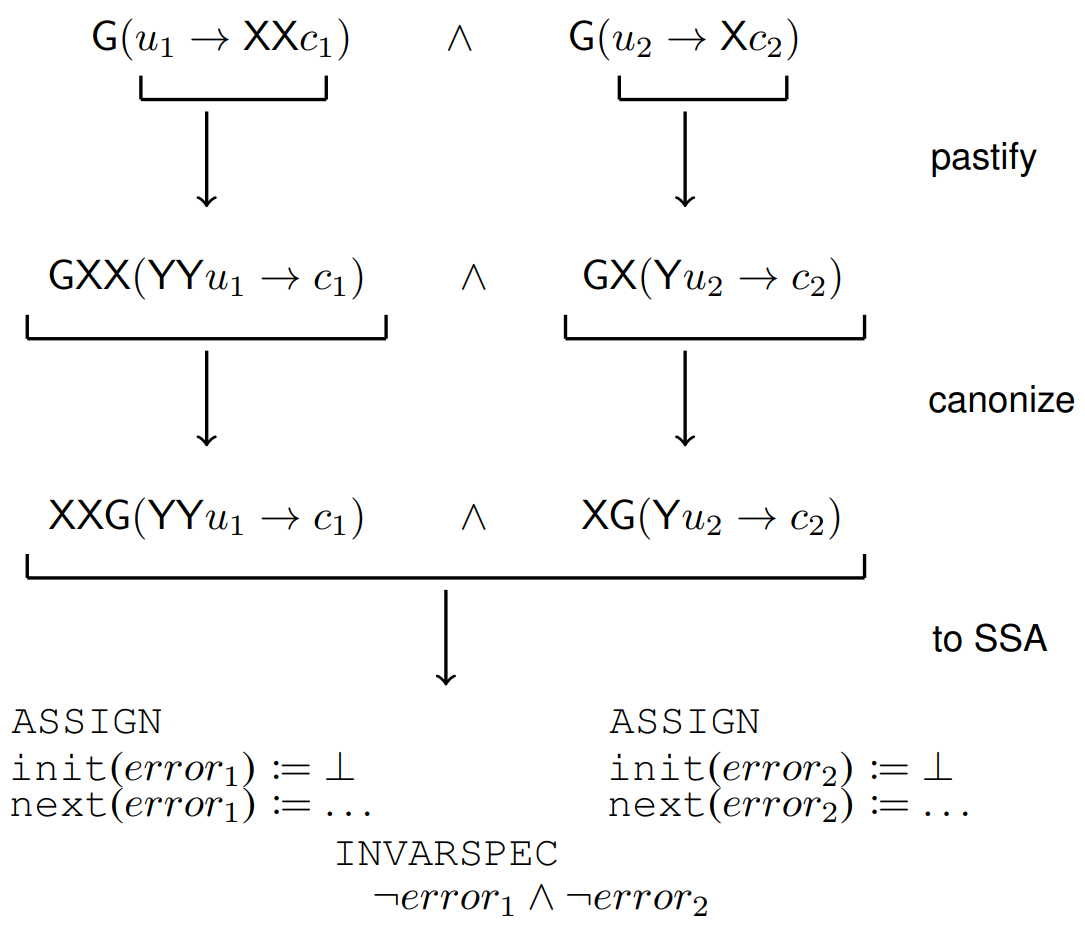
\includegraphics[width=0.6\linewidth]{figures/ebr-ltl-synthesis-example.png}
    \caption{\cite{geatti-2020-08} Example of $\ebrltl$ synthesis for the formula $\ltlAnd{\ltlG{(u_1 \to \ltlX{\ltlX{c_1}})}}{\ltlG{(u_2 \to \ltlX{c_2})}}$}
    \label{fig:ebr-ltl-synthesis-example}
\end{figure}

After having built the automaton, the respective safety game $\game = \tuple{\automaton_\phi, \C, \U}$ is converted to AIGER format and then given as input to the chosen safety synthesizer, completing the process described previously. It has been proved that the overall procedure belongs to $2EXPTIME$ complexity class, while it belongs to $EXPTIME$ if no constants are admitted managing to get rid of an exponential.

\begin{proposition}[\cite{geatti-2020-08} $\ebrltl$ synthesis complexity]
The realizability problem for $\ebrltl$ belongs to $2EXPTIME$. 
If no constant is admitted, it belongs to $EXPTIME$.
\end{proposition}

The $\ebrltl$ synthesis procedure is implemented in nuXmv under the command \lstinline{_ebr2fsmv}, which reads in input a $\ebrltl$ formula and produces the deterministic SSA of such formula. The SSA is represented by functional SMV modules, that is SMV modules characterized by only Boolean state variables and initial states and next transitions defined via \lstinline{init(var)} and \lstinline{next(var)} statements.
The conversion of SSAs from functional SMV to AIGER format is performed by the command \lstinline{fsmv2aig} implemeted in nuXmv.

